\documentclass[dissertation,copyright]{uathesis}
\usepackage[]{graphicx}\usepackage[]{color}
%% maxwidth is the original width if it is less than linewidth
%% otherwise use linewidth (to make sure the graphics do not exceed the margin)
\makeatletter
\def\maxwidth{ %
  \ifdim\Gin@nat@width>\linewidth
    \linewidth
  \else
    \Gin@nat@width
  \fi
}
\makeatother

\definecolor{fgcolor}{rgb}{0.345, 0.345, 0.345}
\newcommand{\hlnum}[1]{\textcolor[rgb]{0.686,0.059,0.569}{#1}}%
\newcommand{\hlstr}[1]{\textcolor[rgb]{0.192,0.494,0.8}{#1}}%
\newcommand{\hlcom}[1]{\textcolor[rgb]{0.678,0.584,0.686}{\textit{#1}}}%
\newcommand{\hlopt}[1]{\textcolor[rgb]{0,0,0}{#1}}%
\newcommand{\hlstd}[1]{\textcolor[rgb]{0.345,0.345,0.345}{#1}}%
\newcommand{\hlkwa}[1]{\textcolor[rgb]{0.161,0.373,0.58}{\textbf{#1}}}%
\newcommand{\hlkwb}[1]{\textcolor[rgb]{0.69,0.353,0.396}{#1}}%
\newcommand{\hlkwc}[1]{\textcolor[rgb]{0.333,0.667,0.333}{#1}}%
\newcommand{\hlkwd}[1]{\textcolor[rgb]{0.737,0.353,0.396}{\textbf{#1}}}%
\let\hlipl\hlkwb

\usepackage{framed}
\makeatletter
\newenvironment{kframe}{%
 \def\at@end@of@kframe{}%
 \ifinner\ifhmode%
  \def\at@end@of@kframe{\end{minipage}}%
  \begin{minipage}{\columnwidth}%
 \fi\fi%
 \def\FrameCommand##1{\hskip\@totalleftmargin \hskip-\fboxsep
 \colorbox{shadecolor}{##1}\hskip-\fboxsep
     % There is no \\@totalrightmargin, so:
     \hskip-\linewidth \hskip-\@totalleftmargin \hskip\columnwidth}%
 \MakeFramed {\advance\hsize-\width
   \@totalleftmargin\z@ \linewidth\hsize
   \@setminipage}}%
 {\par\unskip\endMakeFramed%
 \at@end@of@kframe}
\makeatother

\definecolor{shadecolor}{rgb}{.97, .97, .97}
\definecolor{messagecolor}{rgb}{0, 0, 0}
\definecolor{warningcolor}{rgb}{1, 0, 1}
\definecolor{errorcolor}{rgb}{1, 0, 0}
\newenvironment{knitrout}{}{} % an empty environment to be redefined in TeX

\usepackage{alltt}
\newcommand{\SweaveOpts}[1]{}  % do not interfere with LaTeX
\newcommand{\SweaveInput}[1]{} % because they are not real TeX commands
\newcommand{\Sexpr}[1]{}       % will only be parsed by R


%\documentclass[dissertation,CC-BY]{uathesis}
%\documentclass[dissertation,CC-BY-SA]{uathesis}
%documentclass[dissertation,CC-BY-ND]{uathesis}
%\documentclass[thesis]{uathesis}
%\documentclass[document]{uathesis}

% Package Usage
% These are the packages that we need
\usepackage{booktabs}
\usepackage{graphicx}
\usepackage{natbib}			% natbib is available on most systems, and is
					% terribly handy.
					
%May need to remove! Trying to fix nocite{*} biblography problem:
					% If you want to use a different Bibliography package, 
					% you should be able to, just change this
					% and the \bibliographystyle command below.  Be warned
					% that you may need to do a little hacking to get
					% the REFERENCES item to show up in your TOC.

% Compatibility with the AASTEX package 
% of the American Astronomical Society.
%\usepackage{deluxetable}		% Allows use of AASTEX deluxe tables
%\usepackage{aastex_hack}		% Allows other AASTEX functionality.

% These are other packages that you might find useful.
% For controlling the fonts, see
% http://www.math.uiuc.edu/~hartke/computer/latex/survey/survey.html
% The following is a nice font set:
%\usepackage{mathtime}			% Times for letters; Belleek math.
%
\usepackage{wrapfig}
\usepackage{caption}
\usepackage{subcaption}
\usepackage{tipa}
\usepackage{color,soul}
\usepackage{url}
\usepackage{blindtext}
\usepackage[inline]{enumitem}
\usepackage{breakurl}
\usepackage{mathtools}
\usepackage{amsmath}			% AMS Math (advanced math typesetting)
%\usepackage{lscape}			% Used for making fitting large tables in by putting them landscape
%\usepackage{refs}			
%
% If you are using hyper-ref (recommended), this command must go after all 
% other package inclusions (from the hyperref package documentation).
% The purpose of hyperref is to make the PDF created extensively
% cross-referenced.

%Also works! Change dvips to driverfallback=dvips.
\usepackage[driverfallback=dvips,bookmarks,colorlinks=true,urlcolor=black,linkcolor=black,citecolor=black]{hyperref}


%Works!
%\usepackage[pdftex,bookmarks,colorlinks=true,urlcolor=black,linkcolor=black,citecolor=black]{hyperref}
%HERE IS THE THING THAT NEEDS TO CHANGE TO GET LATEX TO WORK WITH RSTUDIO. USE pdftex instead of dvips.

% Set up some values.
\completetitle{Working Title: Ear Recorded Speech: A novel approach to automatic and human speech recognition}
\fullname{Samuel John Charles Johnston}			% Grad college wants your full name here.
\degreename{Doctor of Philosophy}	% Title of your degree.



\begin{document}
%set_parent(‘/Users/mwilli/Documents/Spring_2017/Dissertation_Document/Dissertation_Working_Directory_Draft/Dissertation_Main.Rnw')




 





\chapter{Ear-Recorded Speech\label{chapter2}}


\section{Introduction}

The initial experiment was a data collection experiment aimed to create a small corpus of speech data recorded under very specific conditions for use in the following two experiments.  Due to the variability of even the same speaker repeating the same sentence, speech critically needed to be recorded from two locations simultaneously: from the mouth, and from the inside of the ear canal.  This would allow for a more accurate comparison of the two signals.

\section{Background}

\textbf{WHEN FINISHED WITH LIT REVIEW, METHODS AND ANALYSIS, FINISH INTRO AND ADD TRANSITION/OPENNING SENTENCE}
The speech vibrations of a person's own voice will propogate throughout the head and body (cf. \ref{fig:bekesyBodyTransfer}).  Of interest for the present study, these waves will pass through the tissue in the head, and enter into the external auditory canal (EAC), where they will be recorded.

\begin{wrapfigure}{L}{0.5\textwidth}
%\begin{figure}
\centering
  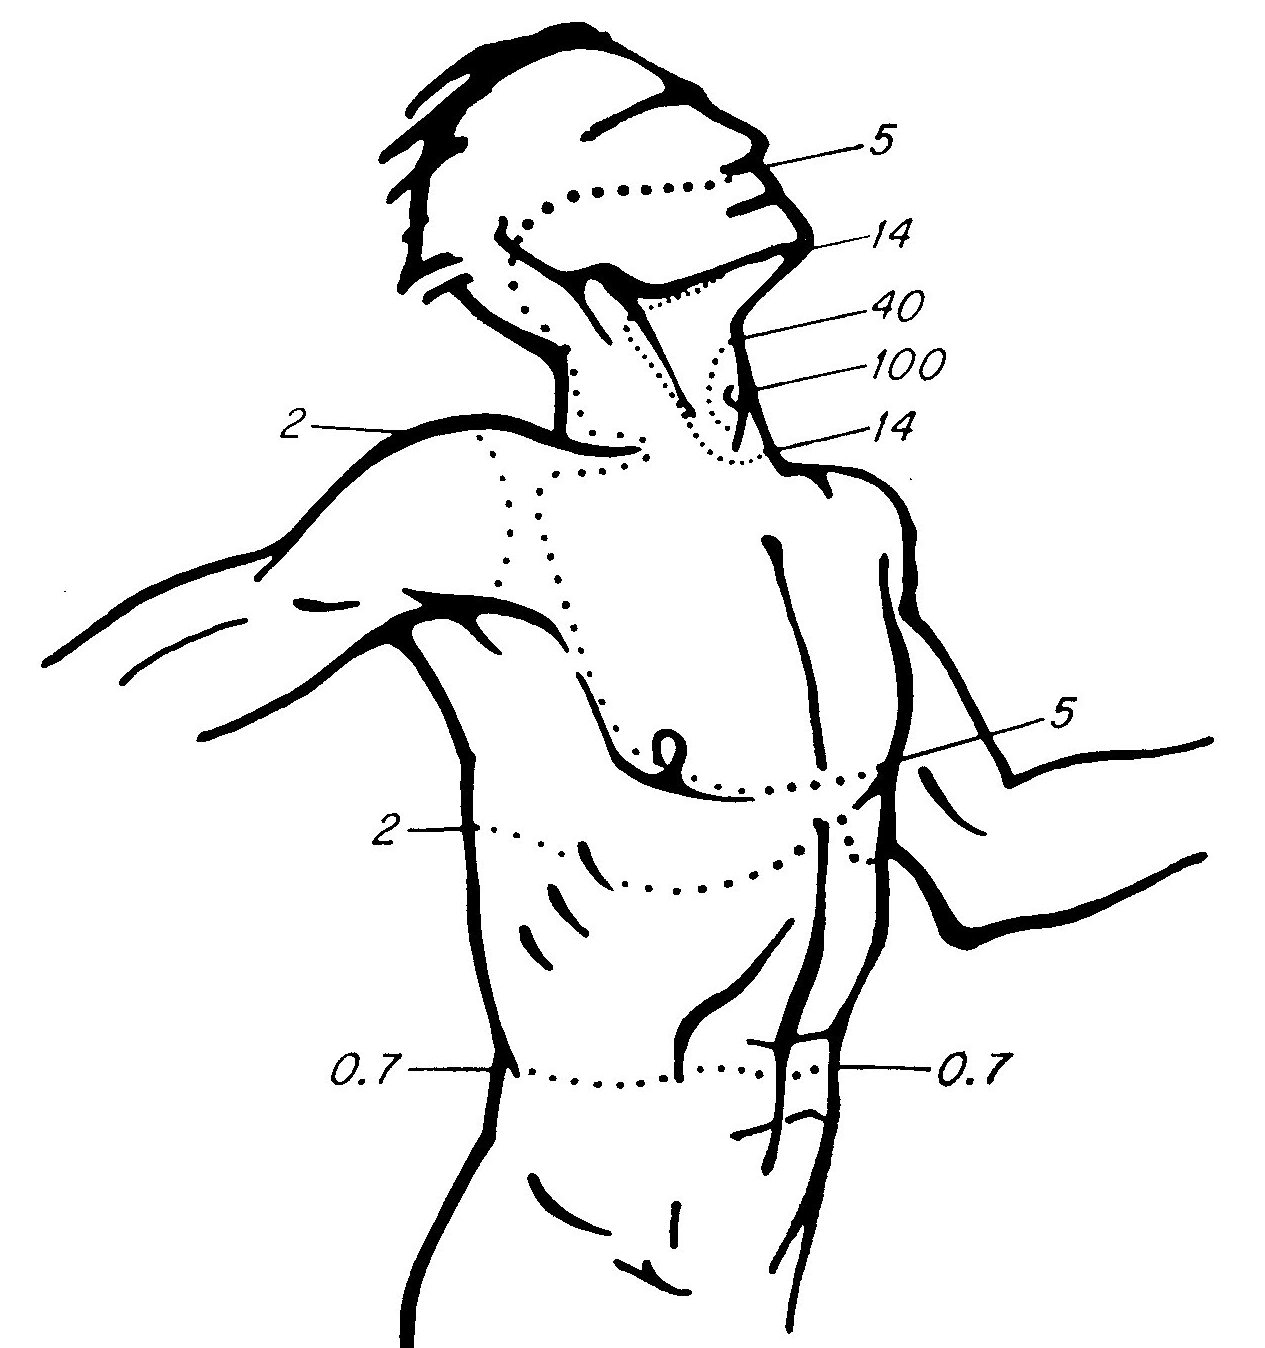
\includegraphics[width=0.5\textwidth]{figure/bekesy60-3b.png}
  \caption{Diagram of the propogation of speech waves throughout the body. Numbers correspond to percentage of the original amplitude of the speech remaining when reaching the marked location. Taken from \cite{bekesy:60}.}
  \label{fig:bekesyBodyTransfer}
%\end{figure}
\end{wrapfigure}

% Discussion about Body/Bone conduction (mechanical)

Bone conduction of acoustic vibrations through a human head has been well studied (cf. \cite{allen:60}, \cite{hakansson:94}, \cite{stenfelt:00}, \cite{reinfeldt:10}, etc); however most of these studies have involved attaching a mechanical vibration device to an animal head or a cadaver skull, or using a vibrating piston on a live human participant, allowing for precise manipulation of the input signal.  
%The acoustic vibrations resulting from the mechanical device positioned on the head propagate to and are recorded by a recording device on a different location on the head.  
Most of these studies, as well, are focused on audiometric bone conduction, i.e. the propogation of waves through the head and their effect specifically on the cochlea itself, which is not relevant to the present study.

%One study, \cite{hakansson}, used ``Live'' human subjects .  Titanium implants (pre-existing) for bone-conduction hearing aids anchored in the temporal bone behind the ear were used as the stimulation point for the mechanical vibrators.
Many of the early studies which were performed on cats do show that the sound generated by bone conduction propogating into the ear canal is dominated by low-frequency noise (\cite{tonndorf:72}).  Normally, the open ear acts as a high pass filter, dampening these lower frequencies passing into it via bone condution.  When occluded, this filter is non existant, and the lower frequencies are more noticeably present (discussed in depth further below). 

Other more recent studies on human subjects have agreed with these findings.  It has also been found that the acoustic response differs significantly depending on the location of the skull that is stimulated\footnote{Typically in these studies it is either the frontal bone or the mastoid process (\cite{bekesy:60}).}.
A few (cf. \cite{bekesy:48}, \cite{hansen:97b}, \cite{porschmann:00}, and \cite{reinfeldt:10}) have investigated body conduction when the source of vibration (i.e. sound) is a person's own voice, not an artificial mechanical vibrator.  These studies also record from the person's ear canal, and not another sensor on a different side of the skull.  

Using speech as a source is inherently messy, because 
\begin{enumerate*}[label={\alph*)}]
  \item  it is not as easily manipulated as a simple mechanical vibrator,
  \item  it has far more frequency components than a simple mechanical vibrator, and 
  \item  it takes multiple pathways to get to the ear: from the vocal chords, through tissue, and into the ear canal, and also from vibrations in the air all along the vocal tract, through the solid medium (although different tissues with different densities) of the head, and back into the medium of air inside the ear canal.
\end{enumerate*}
On top of this, the ear canal itself acts as a resonating chamber (\cite{rosen:91}), altering the signal beyond the distortion already caused by the passage through tissue and bone.  

% Discussion about EAC resonance Theory
% \begingroup
There has been much research on the resonating characteristics and amplitude response of the EAC.  One such project was performed by \cite{stinson:89}, which studied fifteen human ear canals.  Their aim was to produce a model which can replicate the effect that the EAC has on acoustics.
One challenge in producing such a model is the considerable variability in the shape of the canal - both between subjects as well as between the right and left ear canal of a single subject (\cite{stinson:89}).  These differences are apparent in curvature, length, volume, and cross-sectional diameter throughout the EAC.  \cite{stinson:89} created silicon ear molds for each of the ear canals, which were used to generate three different computational models: one following the contours and dimensions of their ear molds exactly, another following the dimensions of the ear mold, but straightening contours and curvatures as if along a central axis, and the third as if the EAC were a uniform tube with the same length and volume of the ear canal molds (and the previous models).  They noted that most significant differences between these models' spectral predictions of EAC resonance occur above 6kHz (see fig. \ref{fig:eac_modelling}).  

Since much of the acoustic information for distinguishing speech sounds is located below 6kHz, several (cf. \cite{stinson:89}, \cite{hansen:97b} \cite{stenfelt:07}) who have made efforts to model the EAC, have chosen to simply treat the EAC as if it were a uniform tube.

Another challenge is to obtain the dimensions of the ear canal needed in order to treat it as a uniform tube in the first place. Immittance measurements are widely used in audiology, and involve emitting a chirp or tone into a pressurized external auditory canal (EAC).  The chirp then bounces back from the tympanic membrane (assumed to have infinite impedance in a pressurized canal) and can be recorded (\cite{ballachanda:97}, 415):``The sound pressure developed inside a rigid cavity from a known sound source is directly related to the volume of the cavity".  Therefore, the volume of the EAC can be inferred for a subject using immittance testing without the need for invasive measurements (e.g. using a silicon mold).  Making an assumption about either an `average' diameter or an `average' length of the ear canal\footnote{The average length of the external auditory canal has been cited from 23mm (\cite{rosen:91}) up to approximately 29mm (\cite{stinson:89}) for a straight tube. The average diameter for the EAC is approximately 7.1 mm \cite{salvinelli:91}.}  would allow for the approximate calculation of the other dimension, given the measured volume. 
%These ear canal dimensions can then be plugged into any one of several models designed to approximate the ear canal dimensions.

\begin{wrapfigure}{L}{0.5\textwidth}
%\begin{figure}
\centering
  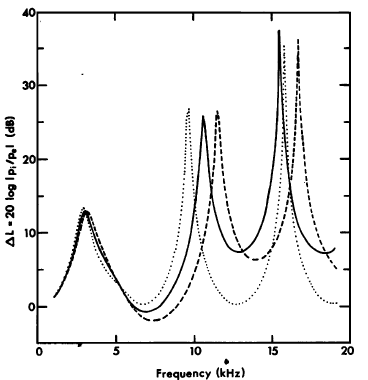
\includegraphics[width=0.5\textwidth]{figure/eac_mod_diffs.png}
  \caption{\cite{stinson:89} diagrams three different models of the external auditory canal (EAC) resonance.  The bold line is based on their 3D canal molds from cadavers, the dashed line removes the curvature of the EAC and acts as if the axis were straight, the dotted line assumes a constant diameter along a straight axis, with the same EAC volume as the dashed and solid lines.}
  \label{fig:eac_modelling}
%\end{figure}
\end{wrapfigure}

% Discussion of the Occlusion Effect

Once inside the ear canal with known approximate dimensions, it can either be modeled as an open-closed tube (if the ear is not plugged) or as a closed-closed tube (if the ear is plugged). This difference changes the resonance and reverberant structure of the external auditory canal (EAC).  This phenomenon, first noted by \cite{wheatstone:79}, is termed the occlusion effect.  The occlusion effect\footnote{The occlusion effect is the change in sound pressure level (SPL) resulting from body conducted vibrations emanating into, and reverberating within, a \textit{closed} ear canal.} offers an amplitude gain to certain frequencies and dampens others.  This has been studied widely and extensively (cf. \cite{wheatstone:79}, \cite{kelly:37}, \cite{littler:52}, \cite{goldstein:65}, among many others).  Generally, the occlusion effect (OE) results in a great increase in the amplitude of frequencies below 1-2kHz, acting as a low-frequency gain and that the amplitude of higher frequencies is dampened (as previously mentioned in the observation in studies of cats\cite{tonndorf:72}).

%\cite{hansen:97b} and \cite{stenfelt:07} are primarily interested in modelling an occluded EAC, and this study requires the model to be a closed-closed tube - that of an \textit{occluded} ear. The models proposed by \cite{hansen:97b} and \cite{stenfelt:07} take many parameters, yet most can be considered to be either \textbf{too difficult to calculate frequently (- what does this mean? give an example)}, or relatively constant (e.g. the impedance of the middle ear, the speed of sound, etc.).  Both models, however, take the parameters for the length of the EAC, the average cross sectional area or diameter, and the volume of the EAC, which, are highly variable.

 
As with bone conduction in general, most of the research of the occlusion effect has been conducted using controlled mechanical vibrations.  Similarly, there is a difference in the OE depending on the location of stimulation.  This difference is most present in the lower frequencies (\cite{dean:00}), where the relative amplitude increase (of body-conducted sound versus air-conducted sound) appears to be the greatest, but tends to wash out when slightly higher frequencies are reached\footnote{\cite{dean:00} found that the greatest relative amplitude increase occurs near 250 Hz, but disappears when 1000 Hz is reached.}.  There are also differences based on the location of \textit{occlusion} within the ear canal, i.e. how deep a plug is placed in the ear canal. \cite{dean:00}'s results indicate this difference does not disappear as frequency increases; the relative amplitude increase is greatest with supra-aural earmuffs at lower frequencies, and lowest with deep inserted earplugs\footnote{\cite{dean:00} does not mention the explicit the depth for each condition, but from the article's description of the insersion procedure, it appears to be ~5mm.}. However, at 1 kHz, the shallow-inserted earplug has a greater relative amplitude gain than the supra-aural earmuff.

\cite{stenfelt:07} developed a model of an occluded ear using measurements generated from stimulating the skull separately at both the frontal bone and the mastoid process.  Each site yielded a slightly different frequency response for the occlusion effect.  Stimulation at the mastoid generally resulted in a greater increase in very low frequencies below 1 kHz.  They also noted that the OE was greatest when using an ear plug near the opening of the ear canal, as opposed to supra-aural `ear muffs' or a deep-insersion ear plug, though an OE was noticeable in each condition; this is in direct contrast with \cite{dean:00}.  \cite{dean:00} do not mention the size of earmuff used, but \cite{stenfelt:07} report the use of a large and small earmuff, with the latter providing a greater OE, though still below that of the shallow-insertion earplugs.
With shallow insersion, their model estimates a gain in amplitude of frequencies below 2 kHz, and dampening of those above; all insersion depths, according to their model, will at minimum, slightly dampen frequencies above 2 kHz.  As the plug is inserted deeper, the damping occurs on lower and lower frequencies.


In contrast to the mechanical source studies above, \cite{hansen:97b} tested the OE using one's own voice as the input source.  \cite{hansen:97b} presents a graph comparing three spectra calculated from continuous speech from three separate publications\footnote{From \cite{wimmer:86}, \cite{thorup:96}, and \cite{may:92}} (Fig. \ref{hansenAverageOEa}).  The study conducted its own tests (seen in Fig. \ref{fig:hansenAverageOEb}), which by and large agrees with the previous measures.  These represent the `average' effect of occlusion on speech, and appears to resemble other (mechanical-source) estimations.  \cite{hansen:97b} developed a model of the OE which largely agrees with these measurements.

The studies looking at human speech result in similar spectral resonances as those dealing with simple mechanical vibrations, except real-speech studies are able to capture the different OE for different kinds of complex sounds in a real speech environment, such as vowels.  

% \begingroup

% \begin{wrapfigure}{R}{1\textwidth}
\begin{wrapfigure}{R}{0.5\textwidth}
\begin{subfigure}{0.5\textwidth}
  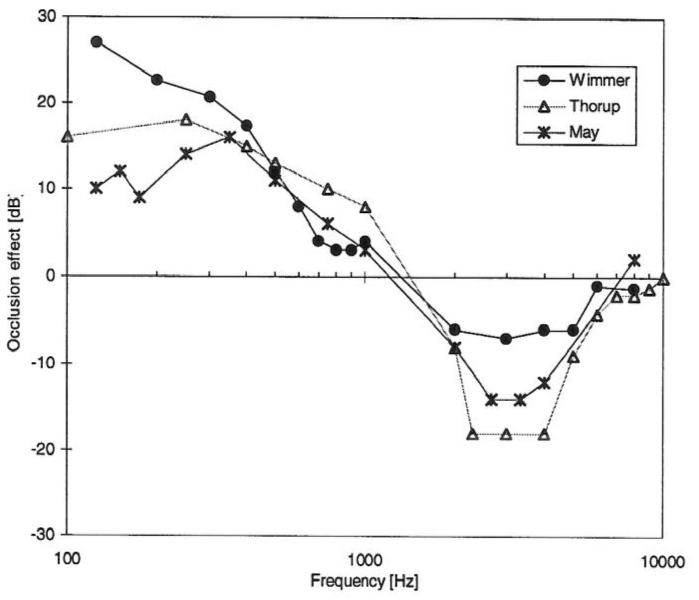
\includegraphics[width=1\textwidth]{figure/hansenAverageOE.png}
  \caption{ }
  \label{hansenAverageOEa}
\end{subfigure}%
\hfill
\begin{subfigure}{0.5\textwidth}
  \begin{subfigure}{1\textwidth}
    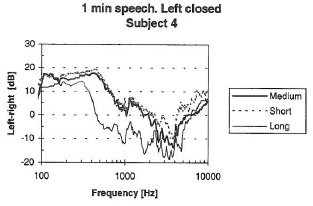
\includegraphics[width=1\textwidth]{figure/Hansen_OE-plot_a.png}
  \end{subfigure}
  \begin{subfigure}{1\textwidth}
    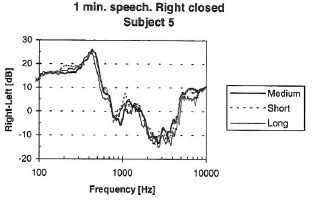
\includegraphics[width=1\textwidth]{figure/Hansen_OE-plot_b.png}
  \end{subfigure}
  \caption{ }
  \label{hansenAverageOEb}
\end{subfigure}
\caption{In (a), three separate measured OE spectra. In (b), a comparison of the occlusion effect (OE) between two subjects (left and right plots) and different sized ear molds that extend into the ear canal at different lengths. Taken from \cite{hansen:97b}.}
\label{hansenAverageOE}
\end{wrapfigure}
% \end{wrapfigure}

%% Allaying concerns of the effect of jaw movement on the occlusion effect.
While \cite{hansen:97b} found phone-specific differences in the occlusion effect (OE), it is ambiguous as to whether the differences are solely due to the differences in the transforms of phones as a result of body conduction, or if there are sound-specific differences introduced within the ear canal or by the occlusion effect itself.  Some have posited that variablility could stem from the fact that the movement of the jaw bone during speech changes the actual shape and size of the cartilage portion of the external auditory canal (EAC) as the jaw moves up and down (\cite{bekesy:60}) for `higher' or `lower' phones (e.g. /i/ vs /a/).  However, \cite{allen:60} studied the occlusion effect (OE) on participants with a unilateral resection of the mandible (one side of the jaw has been removed), and found essentially no distinction between the occlusion effect (OE) in either ear (i.e. with a mandibular joint adjacent to the cartilage of the ear canal or without).


Yet, \cite{hansen:97b}) found that a change in shape of the ear canal due to different jaw positions can create an acoustic ``leak" between the ear canal wall and the occlusion device; the occlusion effect, obviously, behaving differently for different levels of occlusion. 
\cite{hansen:97b} diagrams cross sections of the ear canal with the jaw at different positions; between a closed jaw and 5mm of opening, there is relatively little difference between the shapes of the EAC.  Since \cite{borghese:97} found that the jaw moves relatively little vertical distance during actual speech (max opening approx. 6 mm), it can be assumed that the external auditory canal (EAC) changes shape negligibly during normal speech with a snug-fitting occlusion device. 


% BC + EC resonance (NON-OE)

There have also been many studies (c.f. \cite{bekesy:48}, \cite{porschmann:00}, \cite{reinfeldt:10}) which use real human speech, but rather than isolating the OE, have investigated the output of the entire speech-to-ear canal pathway.

% \begingroup
\cite{porschmann:00} is generally looking at the perception of one's own voice, but in order to accomplish this devotes effort to looking at the bone conduction pathway separately.  A general 900 Hz resonance (with subsequent harmonic resonances) was found in the collected bone-conduction speech, which correlates with the approximately 800 Hz resonances that others  (cf. \cite{tonndorf:97}) have observed in mechanical-stimulated bone conduction studies.  Furthermore, \cite{porschmann:00} notes that there appears to be a general broadband amplitude gain between 0.7 and 1.2 kHz. However, in the study only two phones were used (/s/ and /z/), and a masking threshold \footnote{The masking threshold technique involves playing a pure tone at different frequencies and amplitudes while the participant is phonating. The participant indicates when the tone becomes audible over their own speech, which allows the spectrum of the sound transmission of their speech to be mapped.} technique was used to determine the frequency spectrum of the transfer function of body conduction.  This is admittedly a rather subjective method of determining the spectrum.  

\cite{reinfeldt:10}, on the other hand, uses microphones to record the actual sound pressure level (SPL) of both air and body conducted speech. Furthermore, \cite{reinfeldt:10} used a more expansive and diverse set of phones.  While an overall amplitude gain was found in generally in the same frequency region for /s/ (as well as for several other phones) as that found by \cite{porschmann:00} (0.7 - 1.2 kHz), they discovered a significant sound-class effect (see Figs. \ref{BCrelAC} and \ref{BCrelACall}). Within each class - voiceless sounds (/s/, /t/, /k/, and /tj/),  nasals (/m/ and /n/), and the vowels (/i/, /e/, /a/, /o/) a similar frequency response is seen, yet there are some interesting distinctions to note. These differences can be seen in Figs \ref{BCrelAC} and \ref{BCrelACall}.


% \begin{wrapfigure}{L}{1.1\textwidth}
\begin{figure}
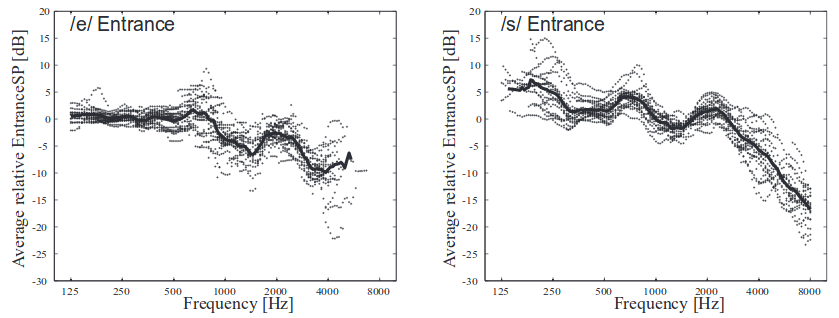
\includegraphics[width=1\textwidth]{figure/BCrelAC_e_s.png}
\caption{Body Conduction relative to Air Conduction for the phones /e/ and /s/.  A value of less than zero indicates the amplitude of body conducted speech is less than that of air conducted speech, and a value greater than zero indicates a higher amplitude of body conducted speech. The solid line indicates the mean, and the remaining data points are from individual speakers.  Taken from \cite{reinfeldt:10}.}
\label{BCrelAC}
\end{figure}
% \end{wrapfigure}

More specific dichotomies can be found between sounds within the same class. For example, the low vowel /a/ is pronounced with a more open mouth vs the relatively closed mouth of the high vowel /i/; consequently, the dB SPL relative to the air conducted counterpart was much higher for /i/ than it was for /a/. An assumption can be made from the data that the more open the mouth is, the more energy is transferred to the air conducted signal (cf. Fig. \ref{BCrelACall}).  This is supported by \cite{bekesy:60}, who also diagrammed the relative difference in amplitude in the ear canal between the air-conduction and body conduction of vowels (cf. Fig. \ref{bekesyPhoneDiff}), which largely supports this hypothesis.  There was much inter-speaker variability, but it appears that the bone-conducted phones with the least relative reduction in amplitude are the higher vowels.  The more energy that is lost to air conduction during the production of low vowels, the less energy is transfered into the surrounding tissue.

\begin{wrapfigure}{L}{0.5\textwidth}
% \begin{figure}
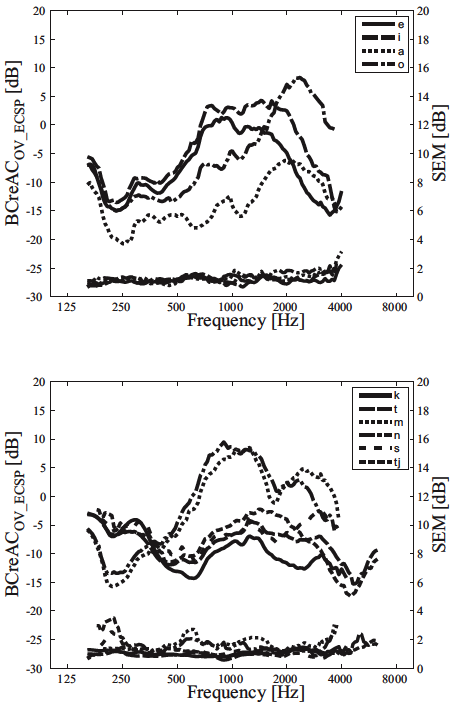
\includegraphics[width=0.5\textwidth]{figure/BC_rel_AC_all.png}
\caption{The mean relative amplitudes (left ordinate) of body conduction relative to air conduction for vowels (top plot) and other sounds (bottom plot).  The set of lines along the bottom of each plot represent the standard error from the mean (SEM), measure on the right ordinate.  Taken from \cite{reinfeldt:10}.}
\label{BCrelACall}
% \end{figure}
\end{wrapfigure}

% \endgroup

% \begingroup
Additionally, \cite{reinfeldt:10} found that the mid back vowel /o/ has a distinctive spectrum in relation to the other vowels, in which there is an amplitude peak near 2 kHz, rather than 1 kHz.  Since the functions of other high back sonorants /u/ and /\textipa{N}/ are not given, we cannot be certain if this is a phone-specific difference, or if it can be generalized to higher ``back" articulations in which the articulatory constriction restricting the acoustic engergy is further back in the vocal tract.\footnote{\cite{bekesy:60} does not break down relative amplitude by frequency}  It is also important to note that these transforms are given as body conducted amplitude \textit{relative to} air conducted amplitude for the given phone, and does not reflect the absolute air- and body-conducted amplitude of phones compared with one another.  For example, /a/ is a relatively loud air conducted sound due to its open articulation, and this loud air conducted component may cause its \textit{relative} body conducted component to appear quieter than the other vowels.  Neither \cite{bekesy:60} nore \cite{reinfeldt:10} give information about body conducted components in relation to one another.


\begin{wrapfigure}{R}{0.5\textwidth}
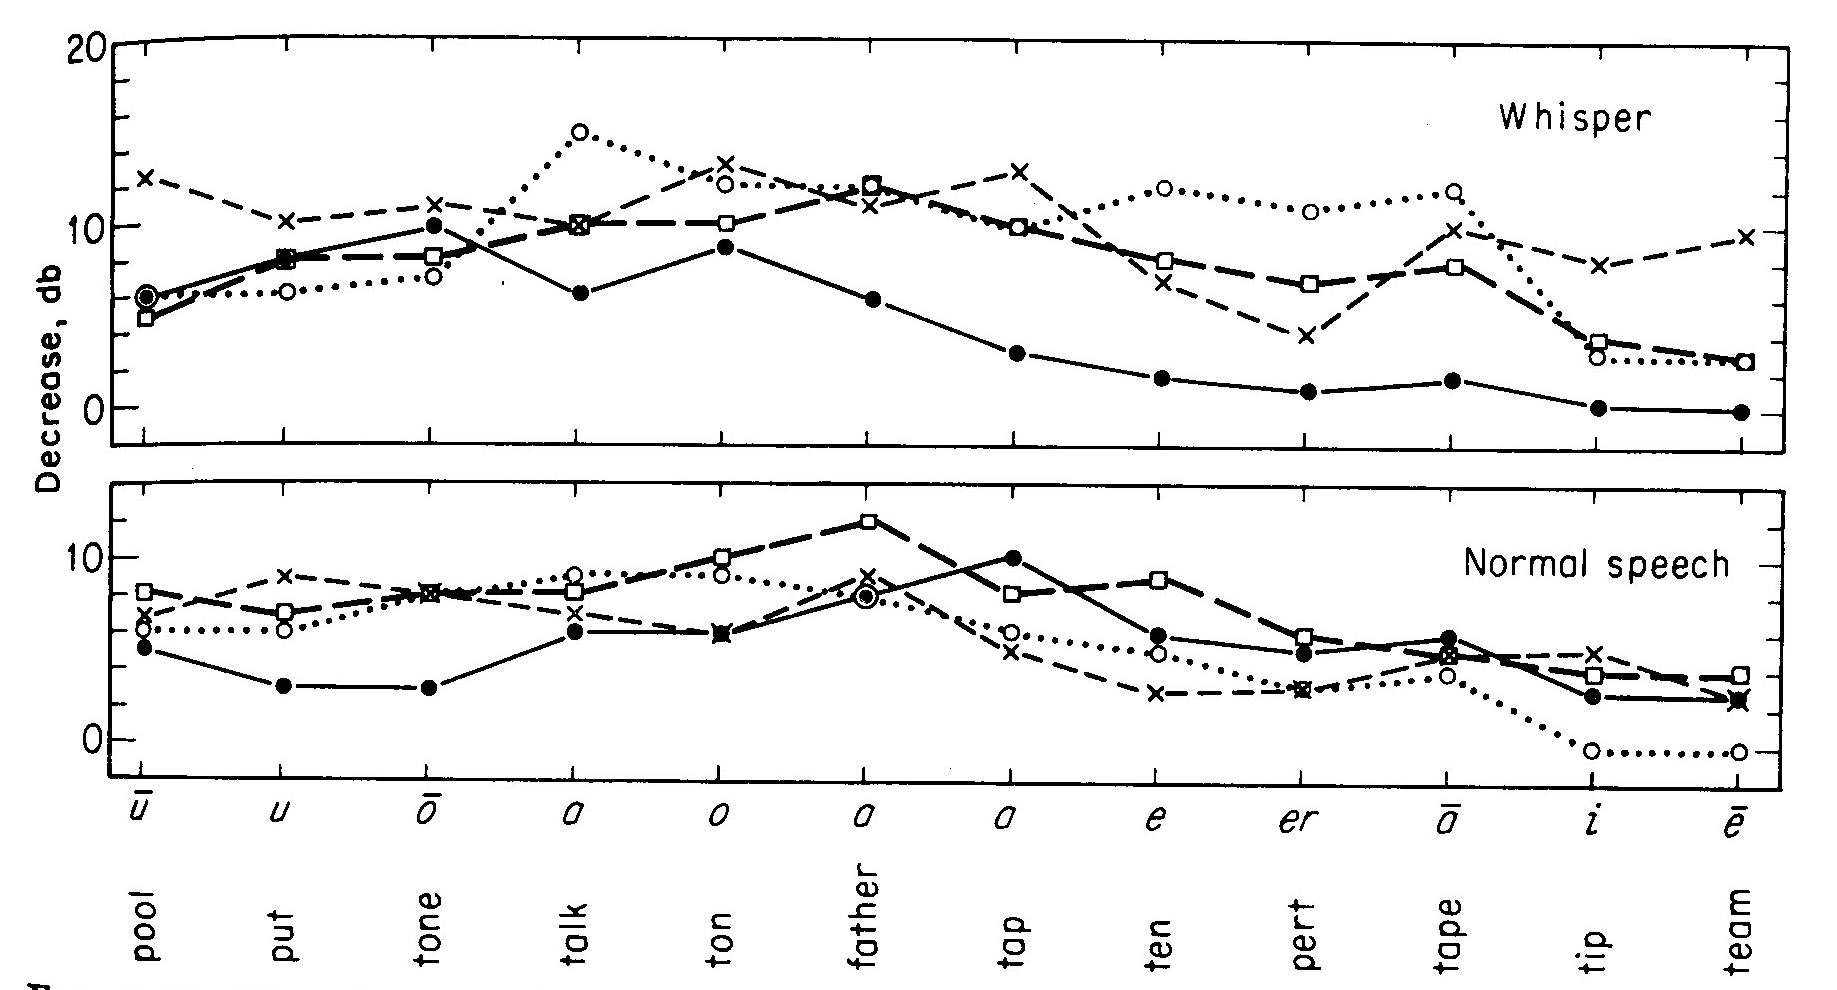
\includegraphics[width=0.5\textwidth]{figure/bekesy60-3.png}
\caption{Demonstrated the different effect on amplitude that closing the ear canal has on the different vowels of English.  Taken from \cite{bekesy:60}.}
\label{bekesyPhoneDiff}
\end{wrapfigure}

% \endgroup

The aforementioned studies on body conduction and the occlusion effect, as would be expected, have indicated a fair deal of inter-person and inter-phoneme variability, and have shown the complexity involved in estimating the effect of body conduction and ear canal reverberance on speech entering the ear canal.  However, the transfer function from the vocal tract to the ear canal does have some standard characteristics, namely, the body and ear canal act as a low-pass filter on speech, removing many of the higher frequencies which are within range of containing critical components for speech intelligibility.

%CONCLUSION to expt 1 lit review

%There is a possibility that the ear signal might be so low-pass filtered as to dampen the upper frequencies beyond retrieval and to the point that accurate recognition is unlikely.  In this case, there are still several possibilities, one of which will be outlined below.  

%While critical speech information may be lost, there is still critical speech information that will be present in the signal, namely the pitch.  The ear signal could be used to ``clean" a simultaneously recorded signal obtained from the mouth (which includes any ambient noise).  Since the occlusion effect acts as a gain in the low frequencies, the harmonic information of the voice signal can be reliably obtained from the ear signal.  Using this harmonic information, a comb filter (cf. \cite{nehorai:86}) could be developed and applied to the noisy mouth signal (cf. \cite{king:08}, \cite{cai:09}, \cite{jin:10}).  The comb filter acts as a series of narrow bandpass filters at equal (harmonic) intervals; when applied to speech, this can filter out the noise located in-between the harmonics.  

%There are a number of drawbacks with this method, however.  One is that this method primarily is used to recover voiced (harmonic) sounds, and fricatives or other voiceless sounds may not be able to be `cleaned'.  Another is that while speech is generally harmonic-like, it is not a perfectly harmonic signal, and there is a possibility that some of the higher harmonics might be accidentally filtered out.  This is particularly concerning as the higher frequencies are what is missing from the ear-recorded signal in the first place.


The methods described in this section, namely the models and transfer functions used by \cite{hansen:97b}, \cite{stenfelt:07}, and \cite{reinfeldt:10}, predict a general rise in amplitude of lower frequencies (below 2 kHz), and a drop in frequencies above that range (with a few exceptions).  This distortion is hypothesized to be predictable, unlike ambient noise from the environment, which is generally highly variable in both amplitude and type.  Due to this, the technique of substituting unpredictable noise with the ``predictable noise" of body conduction and the occlusion effect allows for greater confidence that a usable signal will be recovered.  The ``recovered" signal after undergoing minor transformations is hypothesized to perform better than a noisy signal collected from the mouth in both ASR and human speech perception tasks.  Section \ref{expt1} below describes the specific methods used to collect speech data from the mouth and the EAC and recover an intelligible signal from the latter using the principles outlined in this section.


\section{Experiment 1: Creating a dataset of ear-recorded speech\label{expt1}}

Due to the numerous constraints and requirement for the speech recordings it was necessary to create an original dataset for this study. 

\subsection{Design}
   
The goal of this experiment was to create a dataset of recordings, both from the mouth, in noisy conditions, and from inside the ear in the same conditions.  These recordings needed to demonstrate that (a) by recording speech from the ear, external noise was completely or largely eliminated, while simultaneously recorded speech from the mouth had a noisy background, (b) that the speech from the ear was more intelligible and recognizeable by humans than noisy speech, and (c) that the speech from the ear was more intelligible and recognizeable by an ASR system than noisy speech. 

In alignment with the CHiME challenge\footnote{The CHiME challenge tasks researchers to improve upon or surpass a baseline automatic speech recognizer used on noisy speech data.} guidelines, this study uses different types of background noise at different noise levels.  The noises used include the four sounds (bus, cafe, pedestrian area, \& street) from the CHiME\cite{chimeURL:2016} challenge were used, plus a factory track taken from \cite{factoryURL}.  A short portion of the audio with relatively level amplitude was extracted from each sound file to be played in the background.\footnote{\textbf{The exact portions of these sounds which were used are available online, along with the rest of the data at URL.COM}}

Three noise levels were used.  Since conversational speech is generally around 70 dB, the levels chose were 60 dB, 70 dB, and 80 dB\footnote{These were the `averaged' dB level over the course of the sound file}.  This would result in approximate SNR conditions of +10 (60 dB), 0 (70 dB), and -10 (80 dB).  80 dB was also chosen as a max loudness in order to leave a wide margin between it and any (albeit remote) possibility of hearing damage. A `clean' condition was also utilized (no noise).  Thus far this creates 16 different conditions (5 noise types * 3 noise levels + 1 `clean' condition).  

\subsection{Stimuli}
Thirty sentences were chosen from 3 Harvard Sentence lists\footnote{The `Harvard Sentences' is comprised of 72 lists, each 10 sentences long, where each list of 10 sentences is phonetically balanced, where the proportion of each phone in the list corresponds with it's occurrence in the English language.\cite{harvardSentencesURL}}.  Lists 14, 28, and 57 were used, and chosen semi randomly, eliminating lists with potentially unfamiliar or rare words.  Each sentence occurs in all 16 conditions, resulting in 480 total stimuli.

  
\subsection{Equipment}

The experiment took place in a XXXX soundbooth.  To create the artificially noisy environment a Yamaha MS101 III loudspeaker was hooked to an HP ProBook 6470b laptop.  A sound pressure level meter (SPL meter; Larson Davis Model 831) with a PCB Piezotronics Model 377B20 condenser microphone (omnidirectional) was placed 1 meter from the loudspeaker and measured the sound pressure to verify each of the three noise levels for each of the 5 noise types. A Grason-Stadler GSI Typstar Middle Ear Analyzer was used to measure the ear canal volume and test for plug leaks.  Two Countryman B2D directional lavalier microphones were used to record the mouth speech and the ear speech.  A pair of 3M Professional Peltor Earmuffs with an NRR of -30 dB SPL were worn by the participant during the experiment.  These were hooked up to a PreSonus Digital Audio Firebox preamplifier, which was connected via TRS cables to a Zoom H6 Handy Recorder.


\subsection{Participants}
Twenty participants were used in this study, ten female and ten male, all native speakers of English with normal hearing.

\subsection{Procedure}

The participant is initially asked a few preliminary demographic questions\footnote{e.g. 2nd language (if any), etc. For a list of all information gathered, see \ref{appendixB}.}. They are seated in front of the Middle Ear Analyzer.  An otoscope is used to ensure the ear is mostly free of cerumen, to avoid blocking the microphone off from the rest of the canal or generally impacting the canal with cerumen.  The chosen ear is fitted with an appropriate sized rubber clinical single-use ear tip, into which the Middle Ear Analyser hose is already plugged.  An immittance test is performed, which involved playing a tone, and slightly and briefly pressurizing the ear.  The Middle Ear Analyser checks that the ear plug solidly seals off the ear canal in order to be able to build up pressure, and alerts the researcher to a leak if the plug is not securely in place.  This test results in an estimate of the volume in milliliters (mL) of the external auditory canal (EAC) and of the middle ear, with precision to a tenth of a mL; additionally, a graph of middle ear function is given, which is checked for normalcy (cf. \ref{appendixB}).  Several other measures are given which are not used in this study.

The distance from the end of the ear plug to where it is enclosed by the ear canal is measured to determine how far the plug was placed in the ear canal (cf. Fig. \ref{earplugInserted0.png} for diagram).  Since the length of the plug was known, this was done by placing a measuring rod against the cavity of the concha to measure how far the plug was sticking out of the ear. The decision to treat the cavity of the concha as the ``end" of the EAC is taken from \cite{stenfelt:07}, who made molds of ear canals, and treated the rapid increase in volume (where the cavity of the concha begins) as the end to the EAC.  This measure allows for the calculation of the depth of insersion of the earplug.

The Middle Ear Analyser hose is then taken out of the ear plug - which is carefully left in place to ensure a continuous seal.  The participant then moves to a seat located in front of a computer monitor.  The loudspeaker is on another table to the right of the participant, perpendicular to the direction the participant is facing (cf. Fig \ref{overallSetUp1.png} for set-up diagram).  The participant is then instructed as to the proceedings of the rest of the experiment. One of the two microphones is taken, the wind-break foam removed, and is snugly inserted into the ear plug.  A mark on the microphone cable was used to ensure the end of the microphone was fully inserted to the end of the earplug.  Occasionally, the microphone was inserted deeper than, or just shy of, the end of the ear plug; the variance is within +/-1mm depth (cf. \ref{appendixB}).  The earmuffs are placed over both ears.  Occasionally, a participant had glasses, or thick hair, which may have slightly compromised the seal.  A note was taken of this. 

A wooden rod was attached to the ear muffs, which extends forward, beside the participant's face.  The second microphone was attached to this wooden rod via the lavalier clip at the level of the participant's mouth.  The microphone was directed toward their mouth (cf. Fig \ref{microphoneDetailSetup2.png}).  The placement of the microphone on the wooden rod was adjusted to be exactly 10cm away from the participant's infra-nasal depression.  At this point, the participant was asked to adjust the placement of their chair so that the microphone on the wooden rod was approximately 1 meter from the loudspeaker. Due to the length of the experiment (~45min), no effort was made to discourage minor shifting in body position.  

Both microphones were connected directly to the preamplifier through a fixed (non-changeable) XLR connection.  Both channels were set to the same gain on the preamplifier.  Two TRS cables took each microphone signal from the preamplifier to the recorder.  Both channels were adjusted to appropriate (different) gain levels on the recorder itself to achieve a similar loudness for both signals.  These adjustments were made once the set up was complete, before beginning the recording.

Once recording, an in-house computer program was used to display the stimuli sentences on a second monitor and play the background noises.  For each sentence, the participant saw the clean-condition (no noise) first.  The researcher was in the soundbooth with the participant listening through a pair of headphones connected to the preamplifier.  The participant was asked to repeat the sentence twice to get a rhythm for it, at a normal, conversational loudness, with a normal, declarative intonation.  The researcher asked the participant to repeat the sentence again in this condition if the rhythm of the two statements did not match, or if the participant stumbled over a word.  Each of the following 15 iterations of the sentence (one for each noise-type/noise-level combination) the participant was instructed to speak only once.  If the rhythm of the sentence varied noticeably, or if a sentence was stumbled over, the researcher again asked the participant to repeat the sentence for that condition.  The sentences were not randomized, i.e. all 16 iterations of a sentence occurred consecutively. Within each sentence group (after the first, `clean' condition, which always occurred first), all the conditions were randomized. Each stimulus is advanced by the researcher.

To help the participant notice when a sentence had been advanced\footnote{Wearing the ear muffs, they were not always aware when the noise condition changed.}, the number of the sentence condition was displayed underneath the stimulus (i.e. 1-16).  This had the unindended consequence of occasionally producing a mild list-intonation. 

After the recording was finished, the participant was asked to complete a short, 4 question survey\footnote{cf. \ref{appendixC} for exact (non-coded) survey answers} of their experiences during the experiment.  They were instructed to give as basic or as detailed answers as they wished, but to answer truthfully.  Extra credit in a Linguistics or other participating course was offered in exchange for participation in the experiment.

\section{Experiment 1 Analysis}

Each individual sentence was isolated in each recording with a Praat textgrid and extracted; this resulted in a soundfile for each sentence, for each participant, for both the mouth-recorded and ear-recorded speech.  Figures \ref{spctgrmNarrowMouth_35}, \ref{spctgrmNarrowEar_35}, \ref{spctgrmWideMouth_35}, and \ref{spctgrmWideEar_35} show the narrow and wide band spectrograms for ear- and mouth-recorded speech from participant 35, a female for a ``clean'' example of the sentence ``A cramp is no small danger on a swim''.  These two examples are fairly representative of the speech collected from each location.

\begin{figure}
\centering
\begin{subfigure}{.5\textwidth}
  \centering
  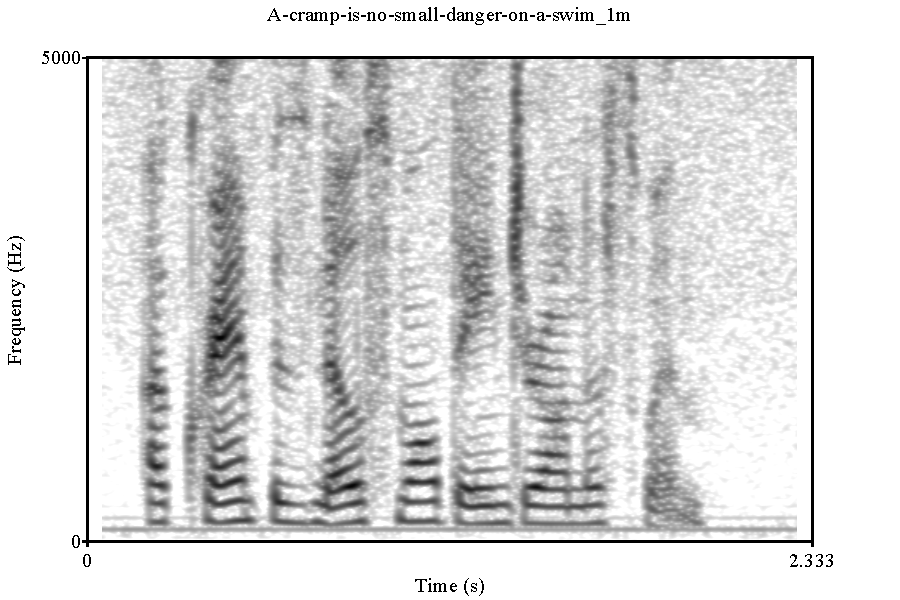
\includegraphics[width=1\linewidth]{figure/spctgrmNarrowMouth_35.pdf}
  \caption{spctgrm Narrow Mouth 35}
  \label{spctgrmNarrowMouth_35}
\end{subfigure}%
\hfill
\begin{subfigure}{.5\textwidth}
  \centering
  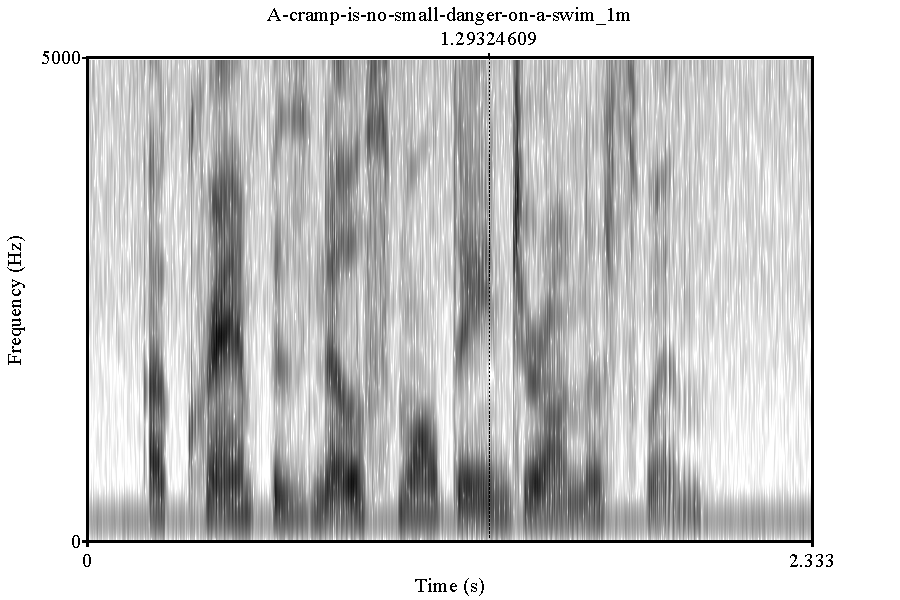
\includegraphics[width=1\linewidth]{figure/spctgrmWideMouth_35.pdf}
  \caption{spctgrm Wide Mouth 35}
  \label{spctgrmWideMouth_35}
\end{subfigure}
\caption{FIGURE CAPTION}
\label{fig:spect_mouth}
\end{figure}


\begin{figure}
\centering
\begin{subfigure}{0.5\textwidth}
  \centering
  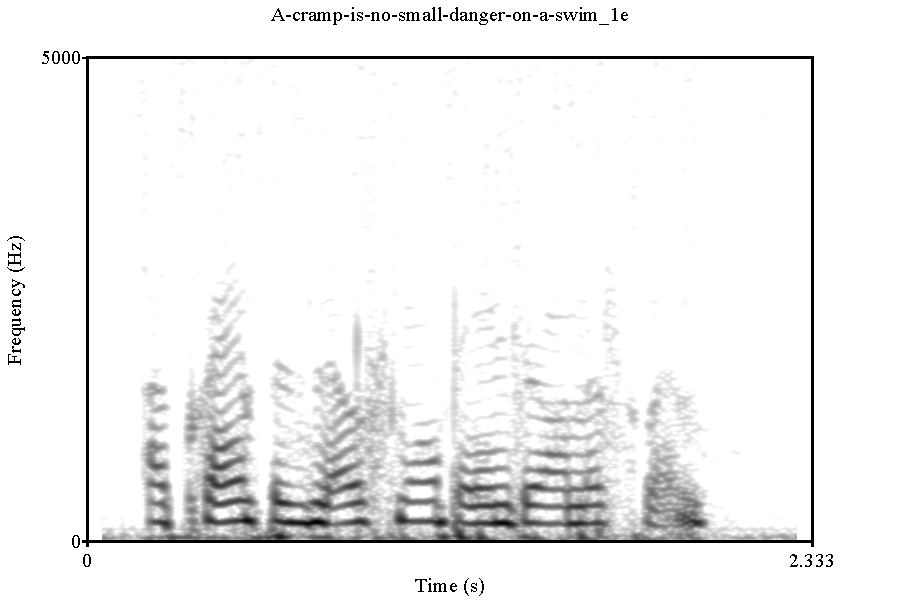
\includegraphics[width=1\linewidth]{figure/spctgrmNarrowEar_35.pdf}
  \caption{spctgrm Narrow Ear 35}
  \label{spctgrmNarrowEar_35}
\end{subfigure}%
\hfill
\begin{subfigure}{0.5\textwidth}
  \centering
  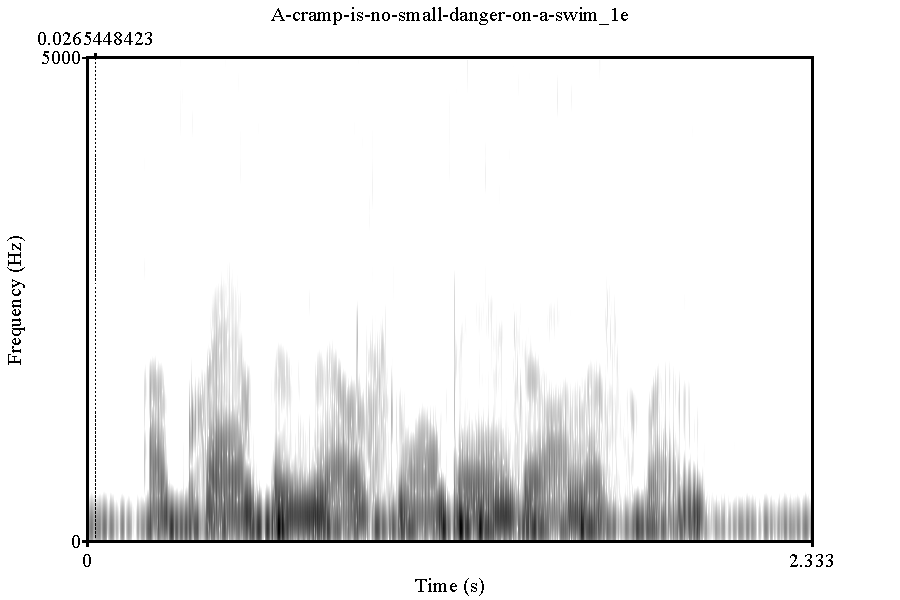
\includegraphics[width=1\linewidth]{figure/spctgrmWideEar_35.pdf}
  \caption{spctgrm Wide Ear 35}
  \label{spctgrmWideEar_35}
\end{subfigure}
\caption{FIGURE CAPTION}
\label{fig:spect_ear}
\end{figure}


As can be seen, the speech collected at the ear is heavily low-pass filtered, and the mouth speech by itself has much more speech information.
However, there are still clear harmonics in the existing range in the ear-recorded speech, and most of the lower two formants can also be seen.

When noise is present, it can be seen in Figs. \ref{spctgrmNarrowMouthNoise_35} and \ref{spctgrmNarrowEarNoise_35} that the noise does not affect the ear recorded signal nearly as much.  There appears to be some of the louder noise (seen in the mouth-recorded speech) present in the upper frequencies of the ear recorded speech, but it is significantly dampened and has a higher speech to noise ratio (SNR).

\begin{figure}
\centering
\begin{subfigure}{0.5\textwidth}
  \centering
  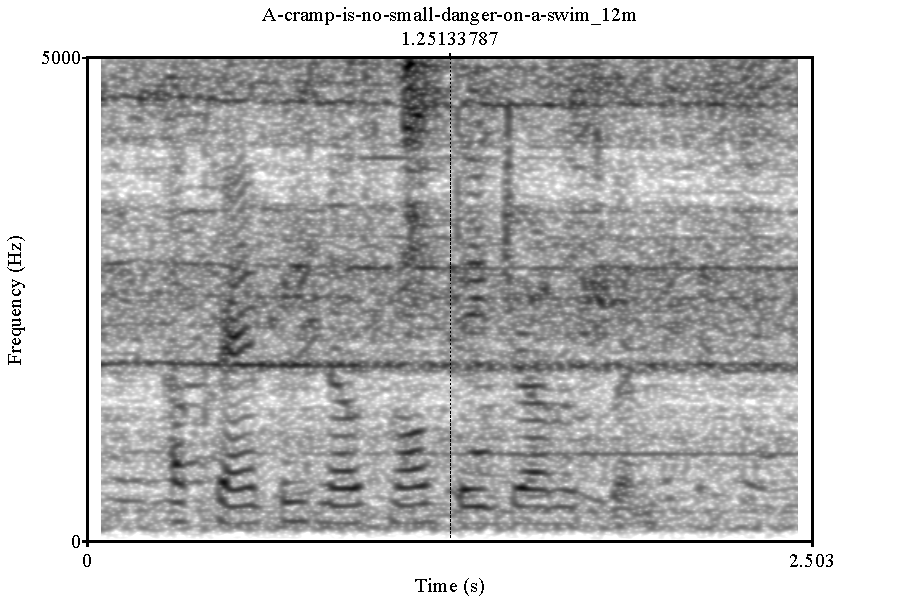
\includegraphics[width=1\linewidth]{figure/spctgrmNarrowMthNoise_35.pdf}
  \caption{spctgrm Narrow Mth Noise 35}
  \label{spctgrmNarrowMouthNoise_35}
\end{subfigure}%
\hfill
\begin{subfigure}{0.5\textwidth}
  \centering
  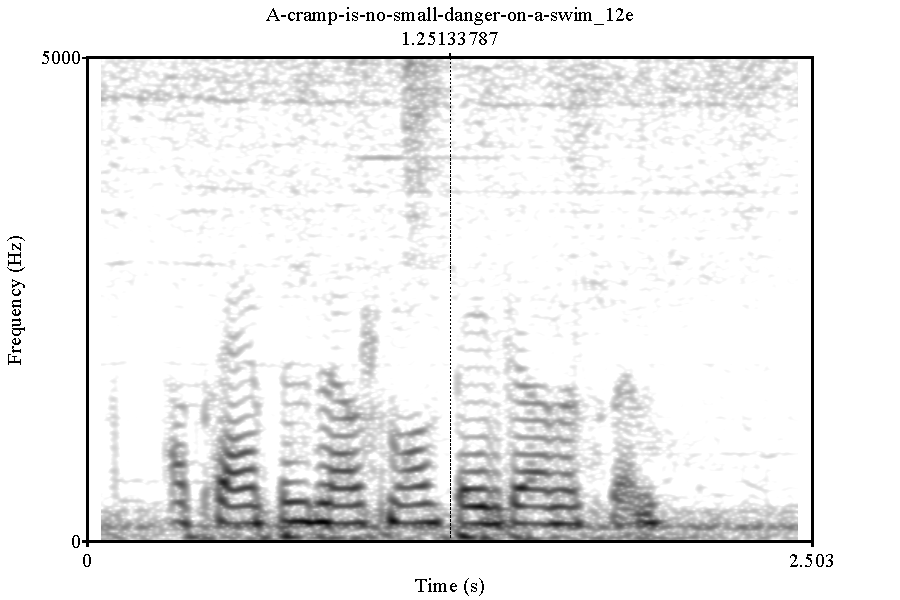
\includegraphics[width=1\linewidth]{figure/spctgrmNarrowEarNoise_35.pdf}
  \caption{spctgrm Narrow Ear Noise 35}
  \label{spctgrmNarrowEarNoise_35}
\end{subfigure}
\caption{FIGURE CAPTION}
\label{fig:noise_mth_ear}
\end{figure}

In an attempt to see if there are recoverable frequencies in the higher ranges, the ear speech was preemphasized, seen in Fig \ref{spctgrmNarrowEarNoisePremp_35}, which has been placed next to its non-preemphasized counterpart for comparison.  It appears that while those fainter harmonics in the midrange frequencies have become more pronounced, there is no new speech information in the upper frequencies which has made it past the noise threshold.

\begin{wrapfigure}{L}{0.5\textwidth}
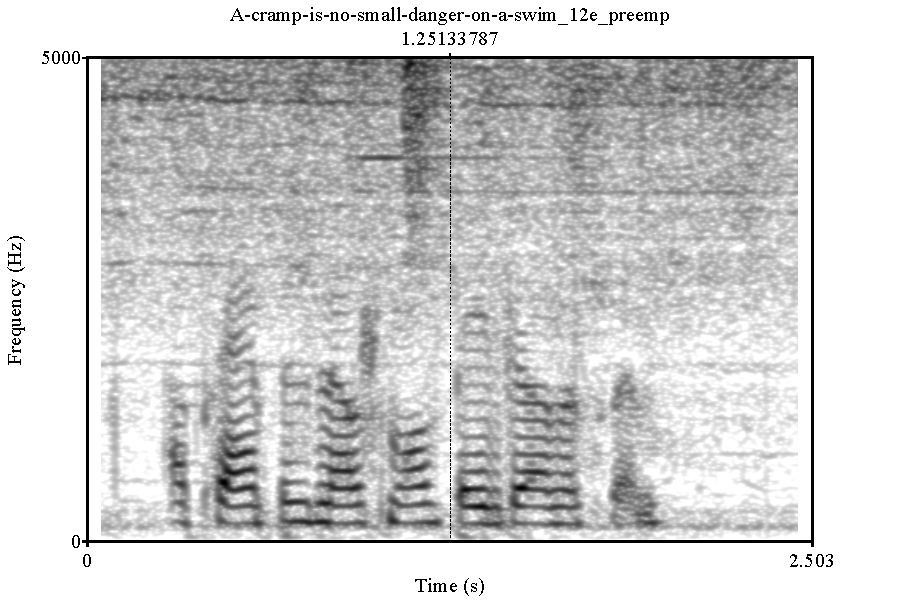
\includegraphics[width=0.5\textwidth]{figure/spctgrmNarrowEarNoisePremp.pdf}
\caption{spctgrm Narrow Ear Noise P 35}
\label{spctgrmNarrowEarNoisePremp_35}
\end{wrapfigure}

This signal was then low-pass filtered at 2500 Hz with a 500 Hz smoothing slope. To further emphasize the higher frequencies (and to smooth over the 'muffled' attribute a bit), the sound was preemphasized a second time (after filtering).  This can be seen in Figure \ref{spctgrmNarrowEarNoisePrempFiltPremp_35}, next to the noisy mouth speech for comparison \ref{spctgrmNarrowMouthNoise_35}.

\begin{figure}
\centering
\begin{subfigure}{0.5\textwidth}
  \centering
  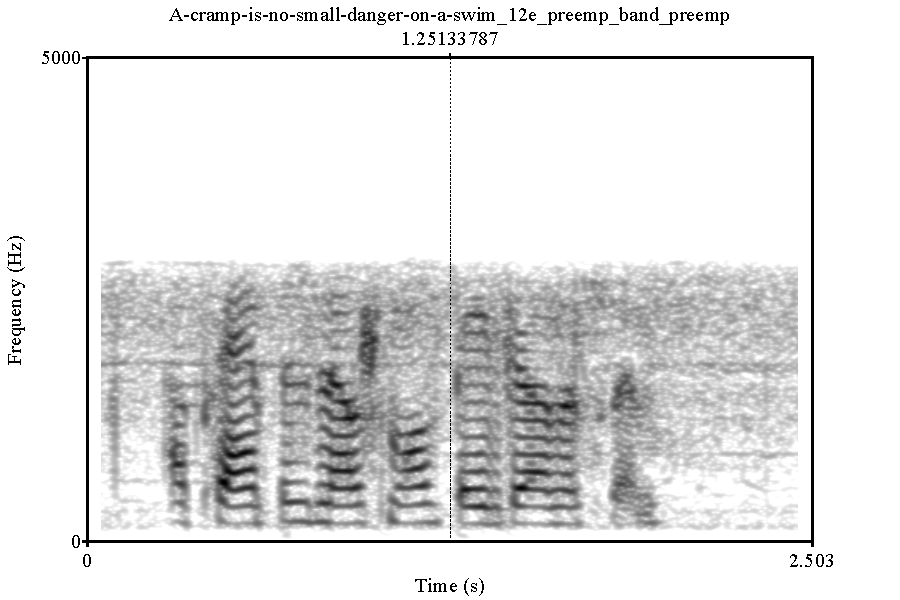
\includegraphics[width=1\linewidth]{figure/spctgrmNarrowEarNoisePrempFiltPremp.pdf}
  \caption{spctgrm Narrow Ear Noise PFP 35}
  \label{spctgrmNarrowEarNoisePrempFiltPremp_35}
\end{subfigure}%
\hfill
\begin{subfigure}{0.5\textwidth}
  \centering
  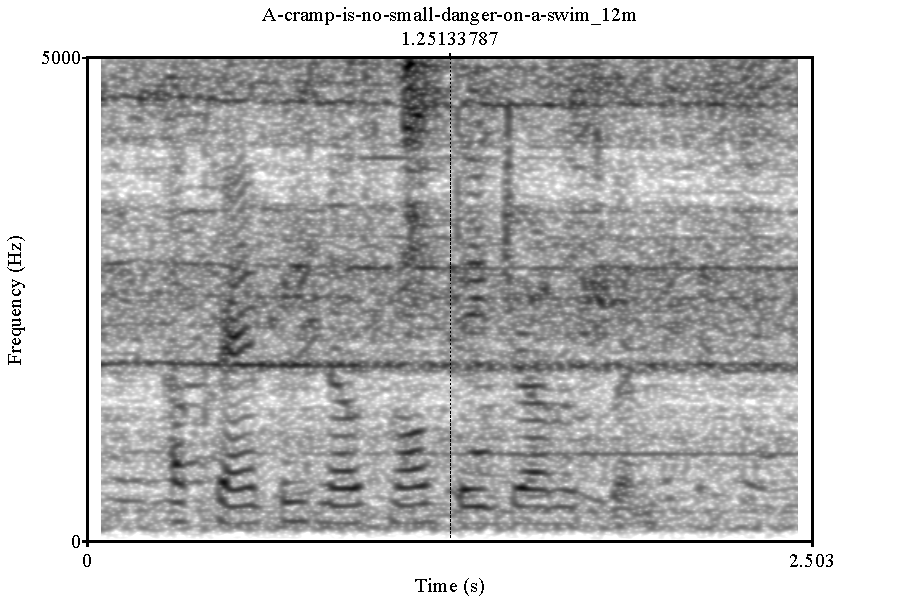
\includegraphics[width=1\linewidth]{figure/spctgrmNarrowMthNoise_35.pdf}
  \caption{spctgrm Narrow Mth Noise 35}
  \label{spctgrmNarrowMouthNoise_35}
\end{subfigure}
\caption{FIGURE CAPTION}
\label{fig:ear_pfp}
\end{figure}

\section{Summary and Discussion}
Here is my summary and discussion. \textbf{Mention the limitations - namely the directionality of the microphone affecting the lack of noisyness in the data}







\bibliographystyle{apa}
\bibliography{DissRefs.bib}
\end{document}
